\section{Conclusions}
\label{sec:adaptui_conclusions}

Inspired by the existing literature approaches for user, context and device
modelling in this chapter a model supported by two main bases has been described.
On the one hand, we have presented AdaptUIOnt, an ontology which deals with the
main problems analysed in Chapter~\ref{cha:state_of_the_art}. On the other hand,
a set of adaptation rules (divided into three groups: pre-adaptation, adaptation
and post-adaptation rules) have been also introduced. These two bases are
illustrated through Figure~\ref{fig:flow_diagram_2}.

The decision of using ontologies is based on the extracted conclusions from the
analysis of the literature. Specially, the analysis by~\citet{strang_context_2004}
is significantly remarked in this dissertation. In this work the authors compare
different context modelling techniques to finally conclude that ontologies
represent the most promising asset with respect to the other analysed techniques
(i.e., key-value models, markup scheme models, graphical models, object oriented
models and logic based models). As the authors state, ontologies are strong
regarding distributed composition, partial validation, content validation
and facing incompleteness and the quality of the information.

Besides, after studying the benefits extracted by~\citet{strang_context_2004}
conclusions and several significant works in the literature (see
Chapter~\ref{cha:state_of_the_art}) we found several more benefits regarding the
AdaptUIOnt model:

\begin{itemize}
  \item It makes the solution more extendible. Knowledge is easily represented
  through semantic models and the models themselves are also easily reusable.
  A context model built by others can be not only use, but for example, extended
  with ambiguity and incompleteness support. In fact, the AdaptUIOnt has been
  built over several contrasted models found in the literature (see
  Section~\ref{sec:adaptui_model}). These models are highly spread and tested
  and due to the nature of ontologies allow us to extend them with our designs.
  
  \item Reasoning is allowed over the knowledge represented in the ontology.
  Ontologies represent knowledge, and one of the benefits of using domain
  concepts is the ability to learn, classify and infer new knowledge from the
  existing one. In AdaptUI there is an architecture module which deals with
  reasoning using the knowledge stored in the AdaptUIOnt ontology (see
  Section~\ref{sec:pellet4android}).
\end{itemize}


\begin{figure}
\centering
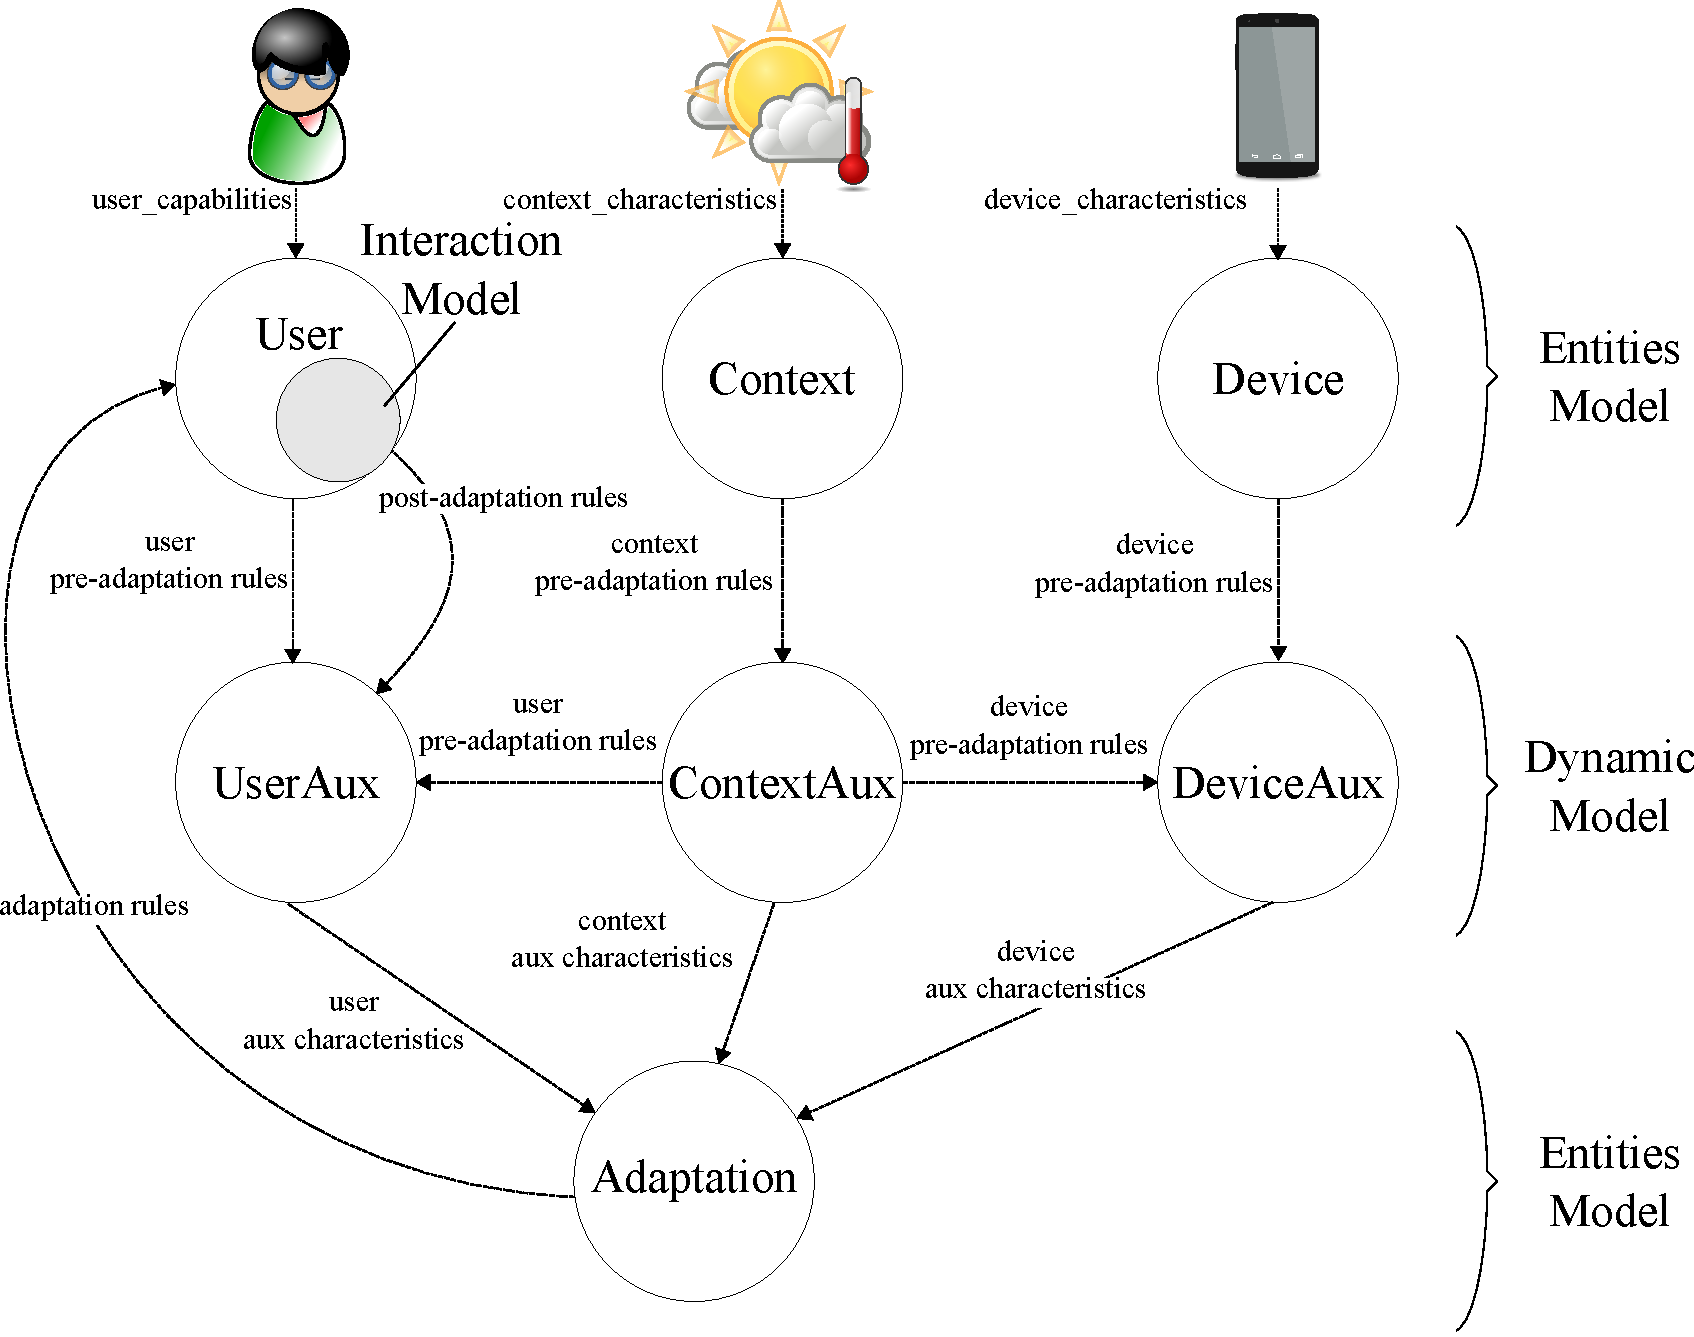
\includegraphics[width=0.75\textwidth]{../figures/PDF/flow_diagram.pdf}
\caption{Knowledge flow through the AdaptUI adaptation process. The circles
represent several main concepts presented in the AdaptUIOnt ontology. The arrows
represent the set of rules that affect the related concepts in the circles.}
\label{fig:flow_diagram_2}
\end{figure}

However, the decision of using ontologies as a modelling technique did not only
bring benefits. The first drawback, and probably the most significant when dealing
with semantics in mobile devices, is the lack of efficiency. Examining several
approaches along the literature we encountered that, usually, the reasoning tasks
are delegated to an external infrastructure. Until the ``smartphones boom'' (see
Figure~\ref{fig:smartphones_boom}) it was quite difficult to find mobile devices
with the appropriate hardware specifications for managing heavy processes. Thus,
the analysed literature approaches usually delegate this processing tasks to
external services (when talking about \acs{ui} adaptation in mobile devices). Then,
these services send back the corresponding results after performing the
corresponding actions. 

This drawback is significant, since AdaptUI aims to not only provide an ontology
model for the adaptation process, but also a series of tools to allow developers
to adapt the ontology and the knowledge represented through it (see Section
~\ref{sec:knowledge_editor}).


\begin{figure}
\centering
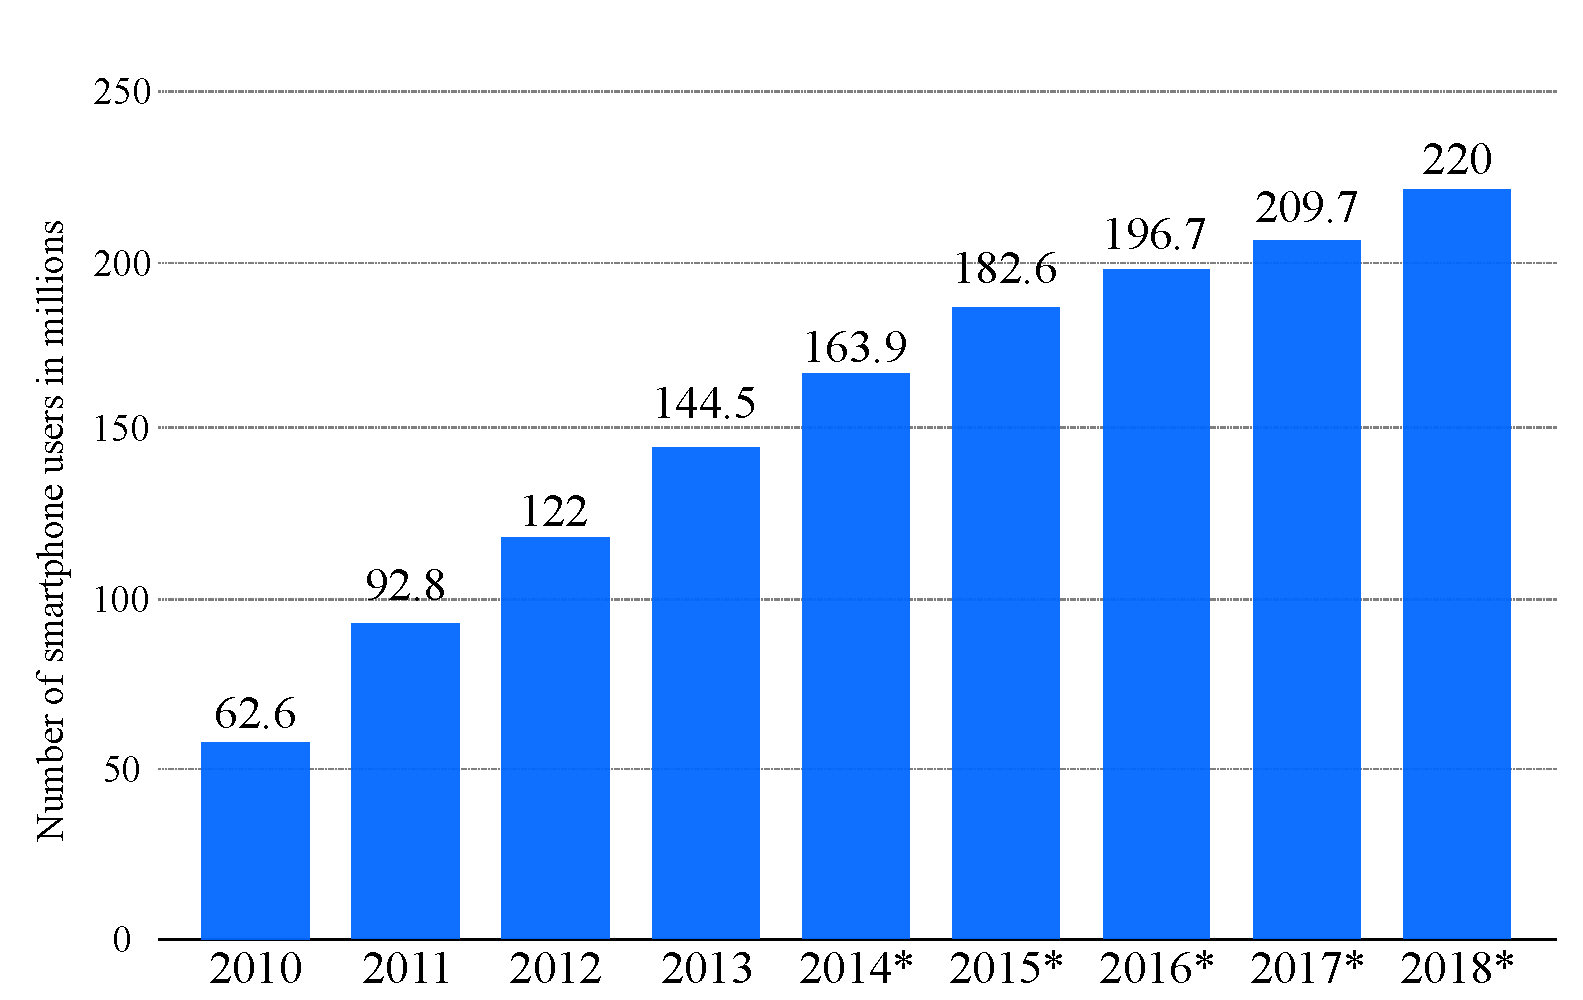
\includegraphics[width=1.0\textwidth]{../figures/PDF/smartphones_boom.pdf}
\caption{Number of smartphone users in the \ac{us} from 2010 to 2018 (in
millions)~\citep{smartphones_boom}. This forecast shows the anticipated number
of smartphone users in the \ac{us} from 2014 to 2018, based on figures from 2010 
to 2013. The source estimates that there will be more than 196 million smartphone
users in the \ac{us} by the year 2016.}
\label{fig:smartphones_boom}
\end{figure}

Another problem deals with the granularity of the model. A generic model might
not be useful for specific scenarios in the same domain, as it would lack specific
parameters. On the other hand, if it is too specific they may not apply well to
other domains. The AdaptUIOnt model tries to address this second aspect by being
abstract regarding the user disabilities. 

Regarding the presented set of rules, it is significant how they represent the
three step adaptation understood by AdaptUI. This is translated into a three
subset of rules which aim to modify and generate new knowledge through a reasoning
process. These subsets, called pre-adaptation, adaptation and post-adaptation rules,
are characterized not only for gathering several rules, but also for being modifiable
by developers through a series of tools provided by the AdaptUI platform. These
tools and their characteristics are detailed in Chapter~\ref{cha:architecture}.